\section{HDR1軸力覚センサの設計}
\subsection{起歪体の構造}
提案する力覚センサの構造をFig.~\ref{fig:sensor}に示す. 

\begin{figure}[b]
  \begin{center}
    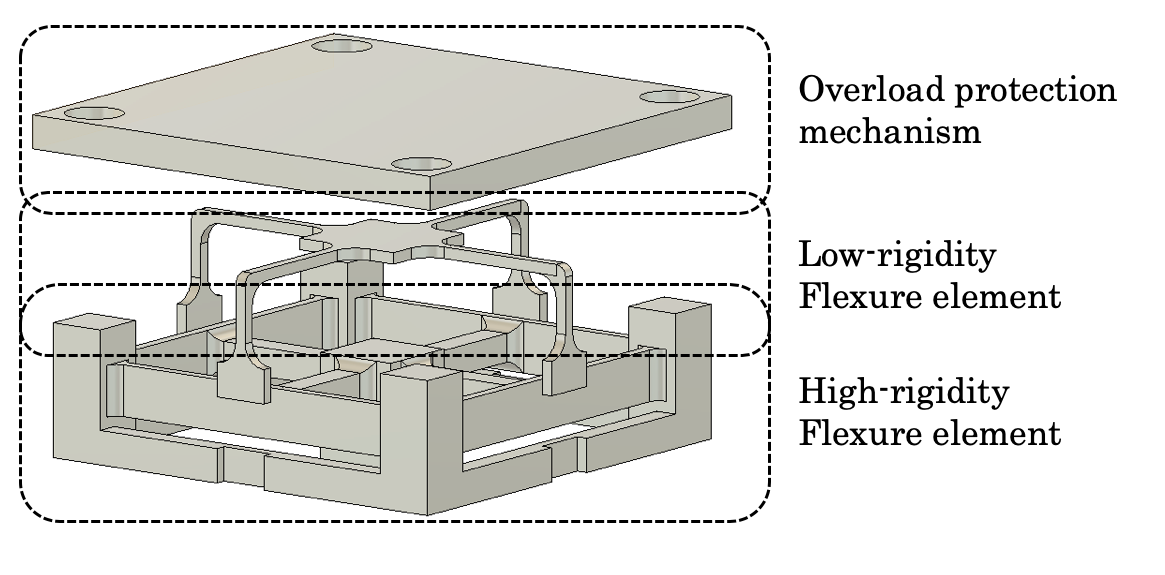
\includegraphics[width=6.0cm]{pic/sensor.png}
    \caption{全体の構造}\label{fig:sensor}
  \end{center}
\end{figure}

提案する力覚センサはセンサは片持ち梁の構造を採用している. 
本力覚センサの設計仕様は有限要素法シミュレーションにより, 
任意の荷重を印加, この時のひずみ, 安全率といったパラメータを参考に決定した.

起歪体の寸法, 定格荷重, 安全率をそれぞれ表○に示す. 
%この時の安全率をTable~\ref{tb:anzen}に示す. 
\begin{table}[h]
  \caption{定格荷重($F$[N], $M$[Nm])}\label{tb:kajuu}
  \begin{center}
   \begin{tabular}{ c c c c c c c }
    \hline
     & $F_x$ & $F_y$ & $F_z$ & $M_x$ & $M_y$ & $M_z$  \\
    \hline
    Low-rigidity & 50 & 50 & 50 & 0.6 & 0.6 & 0.6  \\
    \hline
    High-rigidity & 500 & 500 & 500 & 10 & 10 & 12  \\
    \hline   
   \end{tabular}
  \end{center}
 \end{table}

\begin{table}[h]
  \caption{安全率\label{tb:anzen}}
  \begin{center}
   \begin{tabular}{ c c c c c c c }
    \hline
     & $F_x$ & $F_y$ & $F_z$ & $M_x$ & $M_y$ & $M_z$  \\
    \hline
    Low-rigidity & 2.04 & 2.04 & 1.83 & 1.78 & 1.78 & 3.13  \\
    \hline
    High-rigidity & 1.37 & 1.37 & 1.39 & 1.23 & 1.23 & 1.78  \\
    \hline   
   \end{tabular}
  \end{center}
 \end{table}
%梁は低荷重に対して高感度である必要がある. よって, より細く長い梁が望ましい. 
%しかし定格荷重を印加した時に塑性変形してしまう細さではいけない. 本力覚センサの低剛性起歪体の
%梁の太さは2mm角に設計した. Fig.~\ref{fig:sim}~(a)より印加された荷重に対し
%良好なひずみが得られたことがわかる. さらに, 6成分の定格荷重に対して
%安全率が1以上を確保できている.
%よって設計の妥当性が示された. 

%弾性梁は5mm角で22.5mmの長さ, 弾性薄板は2mm厚, 9mm幅で56mmの長さである. 
%Fig.~\ref{fig:sim}~(b)より印加された荷重に対し良好なひずみが得られたことがわかる. 
%さらに, 6成分の定格荷重に対して安全率が1以上を確保できている. 
%よって設計の妥当性が示された. 

設計した各起歪体の寸法をTable~\ref{tb:size} に示す. 
%\begin{table}[h]
%  \caption{起歪体の寸法[mm]}\label{tb:size}
%  \begin{center}
%   \begin{tabular}{ c c c c c }
%    \hline
%     & & Length & width & Height  \\
%    \hline
%    Low-rigidity & Body & 80 & 80 & 22  \\
%    \cline{2-5}
%     & Elastic bearn & 28 & 2 & 2  \\
%    \hline
%    High-rigidity & Body & 80 & 80 & 23.5  \\
%    \cline{2-5}
%     & Elastic bearn & 22.5 & 5 & 5  \\
%    \cline{2-5}
%     & Thin plate & 56 & 2 & 9 \\
%    \hline
%   \end{tabular}
%  \end{center}
% \end{table}

\begin{figure}[b]
  \centering
  \subfloat[低剛性起歪体]{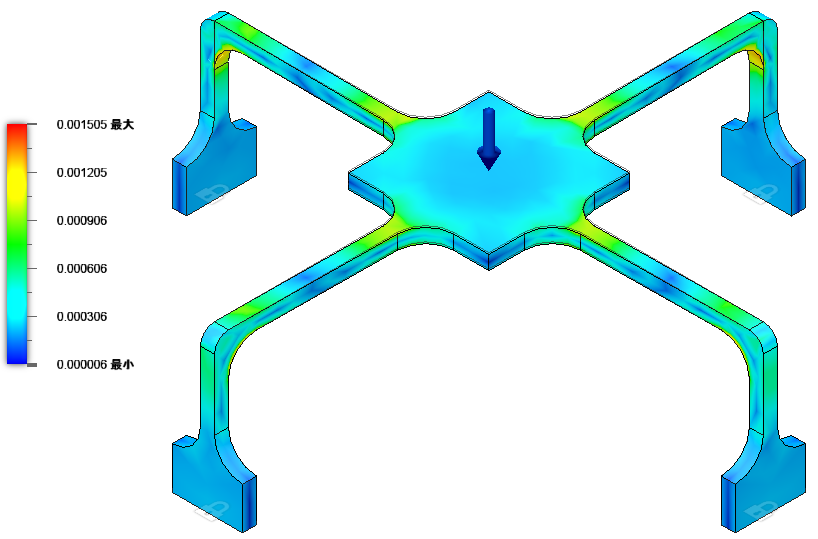
\includegraphics[width=6cm]{pic/Low_sim.png}}\\
 % \subfloat[高剛性起歪体]{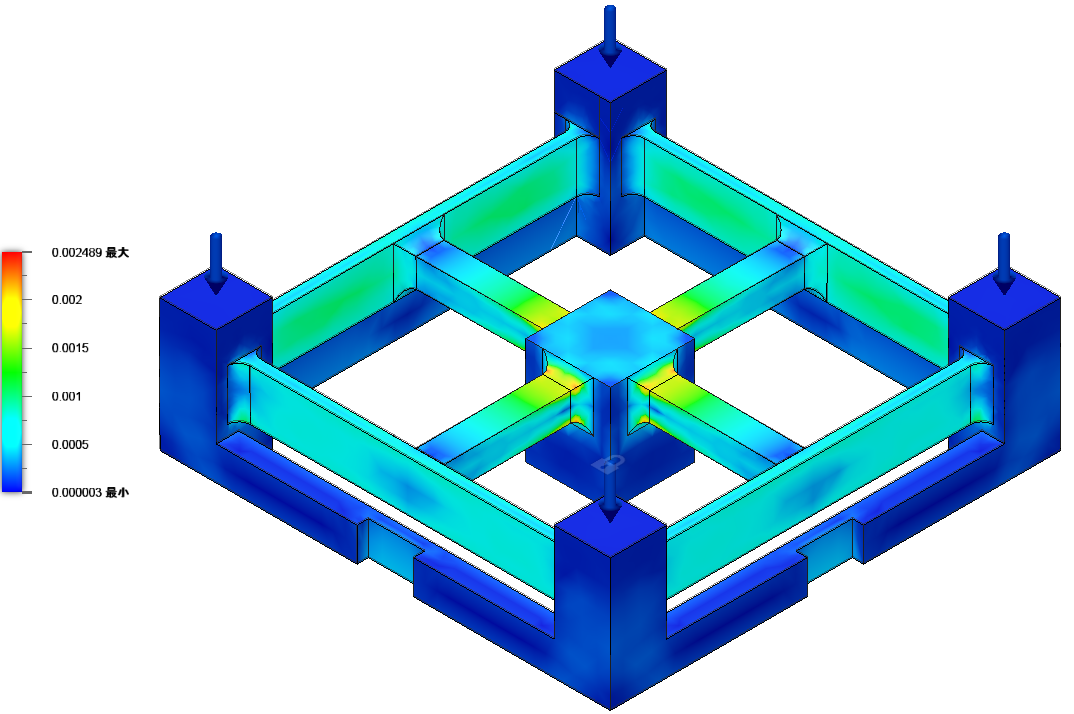
\includegraphics[width=6cm]{pic/High_sim.png}}\\
  \caption[]{有限要素法シミュレーションによる結果}\label{fig:sim}
\end{figure}
\begin{figure}[b]
  \centering
  \subfloat[低剛性起歪体]{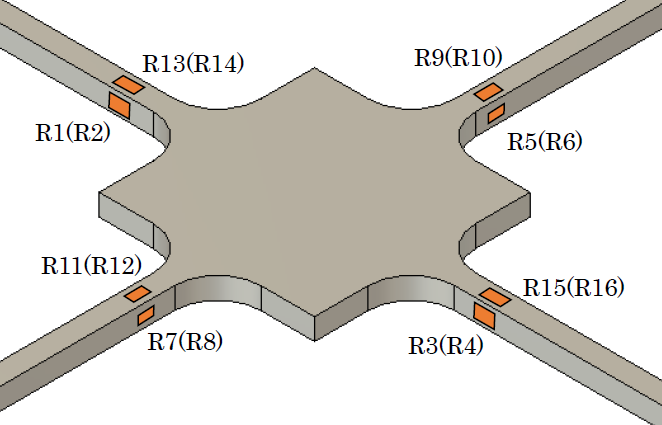
\includegraphics[width=4.3cm]{pic/LowGage.png}}
 % \subfloat[高剛性起歪体]{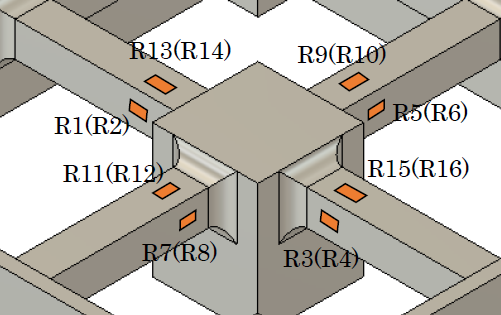
\includegraphics[width=4.3cm]{pic/HighGage.png}}\\
  \caption[]{ひずみゲージの貼付位置}\label{fig:gage}
\end{figure}
